The pipeline is validated at three levels: wire extraction against annotated wire
segments, the Degree-Budget Topology Join against both a real connectivity metric
and synthetic net-level ground truth, and the emitted netlists against a SPICE
simulator. An end-to-end vision-language baseline is reported for context.

\subsection*{Component and wire extraction}

The trained oriented detector reached 88.5\% mAP50 (78.3\% mAP50-95, precision
95.6\%, recall 88.6\%) on the held-out split, with every functional class
detected; the visually hardest class is crossover (70.7\% recall), where two
crossing wires are genuinely ambiguous. On the 134-image evaluation set the
deterministic wire stage achieved a point-based wire F1 of 0.9755 (precision
0.9729, recall 0.9781) in its best configuration. The distribution is strongly
skewed toward clean recovery: the median per-image F1 is 1.000, 117 of 134 images
(87\%) score F1 $\geq 0.90$, and only 4 images (3\%) fall below 0.50 --- dense
layouts where large component occlusion removes wire endpoints.

A thresholding study (Table~\ref{tab:thresholdcomparison}) substituted other
binarization families into the same downstream extraction and evaluation logic.
Sauvola thresholding dominated every alternative: adaptive Gaussian reached
F1 = 0.928, global Otsu 0.828, and triangle thresholding 0.795. Skeleton-based
extraction lost substantial recall by breaking thin wires, and threshold-fusion
variants added nothing over Sauvola alone, confirming that the strong result rests
on conservative local thresholding rather than on any single fusion trick. A
parameter sweep over $k$, window size, link distance, and deduplication angle
moved F1 only marginally, indicating that the extraction stage is robust.

\begin{table}[H]
\centering
\caption{Wire-extraction thresholding comparison on the 134-image benchmark, all run through the identical preprocessing, extraction, and evaluation logic.}
{\small
\setlength{\tabcolsep}{8pt}
\begin{tabular}{p{6.0cm}c}
\toprule
Thresholding family (best setting) & Wire F1 \\
\midrule
\textbf{Sauvola} ($k=0.285$, $w=67$, anchor dist.\ 16) & \textbf{0.9755} \\
Sauvola (baseline, anchor dist.\ 12) & 0.9730 \\
Adaptive Gaussian & 0.928 \\
Global Otsu & 0.828 \\
Triangle & 0.795 \\
\bottomrule
\end{tabular}
}

% 134-image benchmark, identical preprocessing/extraction/evaluation across rows.
% Best Sauvola config (a16): precision 0.9729, recall 0.9781. Sauvola dominates;
% skeleton-based and fusion variants lose recall by breaking thin wires.

\label{tab:thresholdcomparison}
\end{table}

\subsection*{Topology join}

The central result is the connectivity gain from the Degree-Budget Topology Join.
Connectivity is measured as the fraction of components placed on a net shared with
at least one other component; a fragmented circuit scores low because its pieces
are electrically isolated and cannot be simulated. Relative to the endpoint-graph
base join, the degree-budget completion raises connectivity from 68.8\% to 81.9\%
(Table~\ref{tab:mainresults}) and does so without a single per-image regression:
every image is recovered at least as well as the base join. The connectivity gain
comes from a sharp reduction in floating component terminals: the completion
reconnects terminals the detector had left dangling. The one-edge-per-terminal
degree budget and the self-loop guard bound the cost of this recovery, and on the
synthetic net-level ground truth (below) the join's precision does not fall, which
indicates the recovered connections are genuine rather than over-merges. On the
densest real layouts the completion can still introduce a small number of
two-terminal self-loops; this residual cost is discussed in the Limitations.

\begin{table}[H]
\centering
\caption{Topology-join comparison. Connectivity is the fraction of components on a multi-component net; self-loops count two-terminal parts shorted onto one net; regressions count images where connectivity falls below the base join.}
{\small
\setlength{\tabcolsep}{6pt}
\begin{tabular}{p{4.6cm}cccc}
\toprule
Join strategy & Connectivity (\%) & Regressions & Synthetic F1 & Clean F1 \\
\midrule
Endpoint-graph base (\textit{graph\_rescue}) & 68.8 & --- & 0.944 & 1.000 \\
\textbf{Degree-Budget Topology Join} & \textbf{81.9} & \textbf{0} & \textbf{0.969} & 1.000 \\
\bottomrule
\end{tabular}
}

% Connectivity: fraction of components on a multi-component net (134-image set,
% per paper/DECISIONS.md). Regressions: images where the degree-budget join scores
% below the base. Synthetic F1: mean across-severity component-connectivity F1 on
% the synthetic ground-truth harness. Clean F1: round-trip F1 on error-free maps.

\label{tab:mainresults}
\end{table}

Because the real connectivity metric is structural and cannot certify that a
recovered connection is the \emph{correct} one, the join was also scored against
net-level ground truth on the synthetic harness. On a catalog of authored circuits
spanning series, parallel, bridge, multi-source, and adjacent-loop topologies, the
clean (error-free) coordinate maps round-trip to a component-connectivity F1 of
1.000 for the join, confirming the layouts and the join logic are sound. Under the
injected detector-style error, the degree-budget join attains a mean
across-severity F1 of 0.969 versus 0.944 for the endpoint-graph base; it wins at
every severity, and its advantage is concentrated in the dropped-wire regime,
where the completion recovers connections that no purely geometric join can. This
is consistent with the real connectivity gain and indicates the gain reflects
recovered true connections rather than over-merging.

\subsection*{SPICE simulation}

Netlists emitted by the pipeline simulate under \texttt{ngspice}: DC
operating-point analysis returns node voltages and device currents that obey
Kirchhoff's current law on the validation circuits. The synthetic harness provides
a stronger check --- it supplies an analytic operating point for each authored
circuit --- and the simulated source currents match the authored values for every
clean circuit (for example, an authored voltage divider returns its exact
divider current). The same harness shows the qualitative payoff of the join: a
circuit that is fragmented by a dropped wire simulates as dead, whereas after
degree-budget completion it simulates to the correct operating point.

\subsection*{Vision-language baseline}

To test whether an off-the-shelf model could replace the structured pipeline, a
strong vision-language model (Mimo~2.5) was prompted to read the schematics
directly and emit structured connectivity. On 10 representative images it missed
between 38\% and 94\% of the topology, producing plausible-looking but
electrically wrong netlists. The failure mode is informative: the model recognizes
components and the gist of the drawing but does not reliably track which terminals
are electrically common, which is exactly the problem the Degree-Budget Topology
Join solves explicitly and inspectably. (We note that the repository's general VLM
utility defaults to a different model for paper-type classification; the end-to-end
topology baseline reported here used Mimo~2.5.)

Representative pipeline stages are shown in Fig.~\ref{fig:qualitative}: for each
example the input image, the cropped region after component and text suppression,
the Sauvola wire mask, and the final prediction overlay are shown, so that the
effect of each stage can be inspected directly.

\begin{figure}[H]
\centering
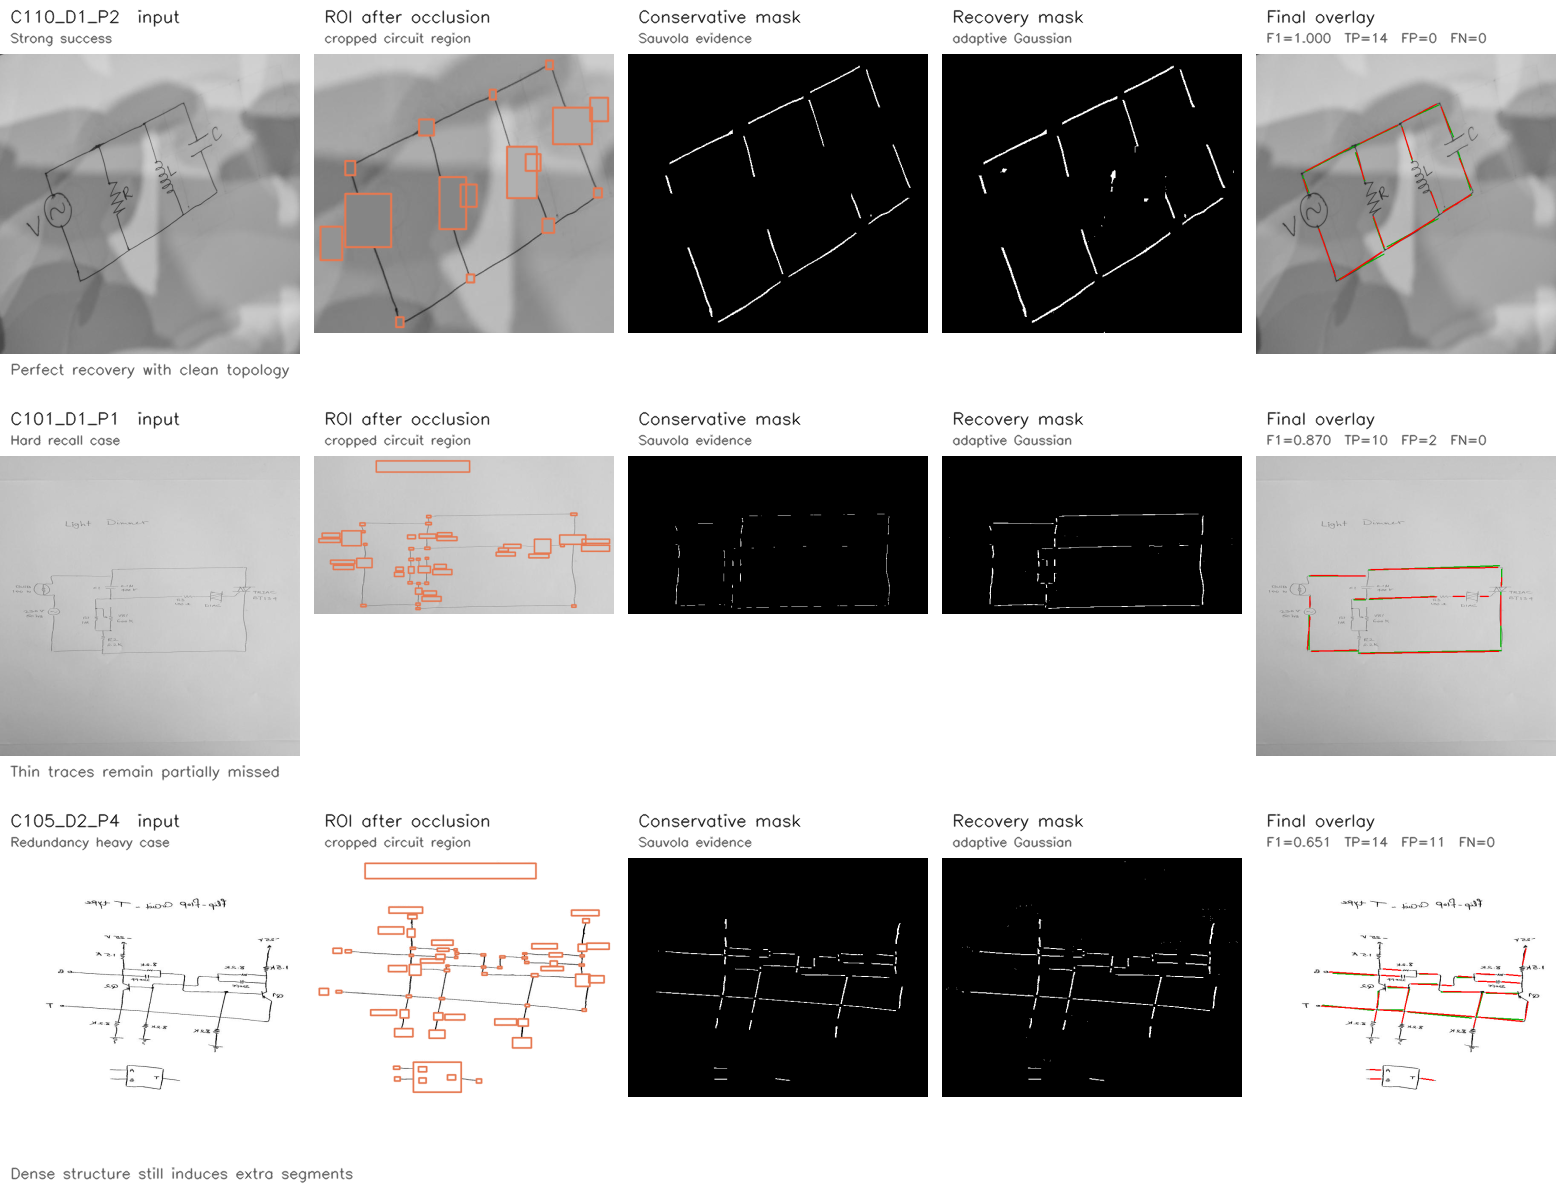
\includegraphics[width=\textwidth]{figures/qualitative_cases.png}
\caption{Representative pipeline stages. For each example the input image, the
cropped region after component and text suppression, the Sauvola wire mask, and
the final prediction overlay are shown. Green segments denote ground truth and red
segments denote predicted wire segments.}
\label{fig:qualitative}
\end{figure}
